\chapter{Arkitektur}
Dette afsnit vil forsøge at beskrive de valg der blevet foretaget ifht. arkitekturen bag BargainBarter. Der vil kort blive beskrevet om de enkelte begreber og arkitekturstile der anvendt til at opbygge systemet og hvorfor disse er valgt.

\section{Arkitektur stile}
Da der i dette projekt ønskes at skabe en webapplikation, så er derfor nødvendigt at anvende den arkitekturstil, der fungerer bedst til dette formål. 
Valget faldt på 3-lags modellen, da denne model oftes anvendes i forbindelse med hjemmesider, da disse består af
\begin{enumerate}
	\item en front-end web-server der leverer statisk eller dynamisk materiale - dvs. al det materiale der vises via webbrowser
	\item et lag der generer og processere  dynamisk materiale 
	\item en back-end database til at gemme og hente data fra
\end{enumerate}
Desuden sørger modellen for at der er lav kobling mellem de forskellige dele. Denne model består af et Presentation Layer, Business Logic Layer og et Data Access Layer. Denne model gør det muligt at skifte de forskellige lag ud, hvis det skulle vise sig at være nødvendigt. Det betyder desuden også at det er nemmere at teste de forskellige dele af systemet. \\
For yderligere information henvises der til dokumentation.

\section{Teknologivalg}
I denne sektion vil der blive beskrevet de specifikke teknologier der er anvendt i projektet.

\subsection{ASP.NET MVC}
Frameworket ASP.NET MVC fra Microsoft blev valgt som platform til webapplikationen, da dette framework har utallige fordele i forhold til dette projekt. 
\begin{enumerate}
	\item Det er skrevet i C\#, hvilken gruppen har stor erfaring i.
	\item ASP.NET MVC er baseret på .NET frameworket og har derfor et stort udvalg af forskellige software biblioteker 
	\item Frameworket har eksisteret i mange år og der findes derfor god support til det
	\item Gruppen har modtaget undervisning i ASP.NET MVC
\end{enumerate}
Der er desuden en masse andre framework, der kunne have været interessante at anvende, såsom Ruby on Rails, men disse framework anvender ikke .NET eller C\#, hvilket gruppen har opnået god erfaring med.

\noindent På figur \ref{fig:MVC} kan der ses den overordnet struktur af den 3-lags model ASP.NET er bygget på. 
Model er den del der arbejder med den data relaterede logik, dvs. Data Acces Layer. Det er altså al den data der tages fra databasen og bliver manipuleret af Views eller Controllers.
View er den del der arbejder på præsentations logikken.
Controller er den del der fungerer som bindeled mellem Model og Views, dvs. den manipulere data ved at bruge Model og interagere med Views for at vise outputtet. \\ 

\begin{figure}[H]
	\centering
	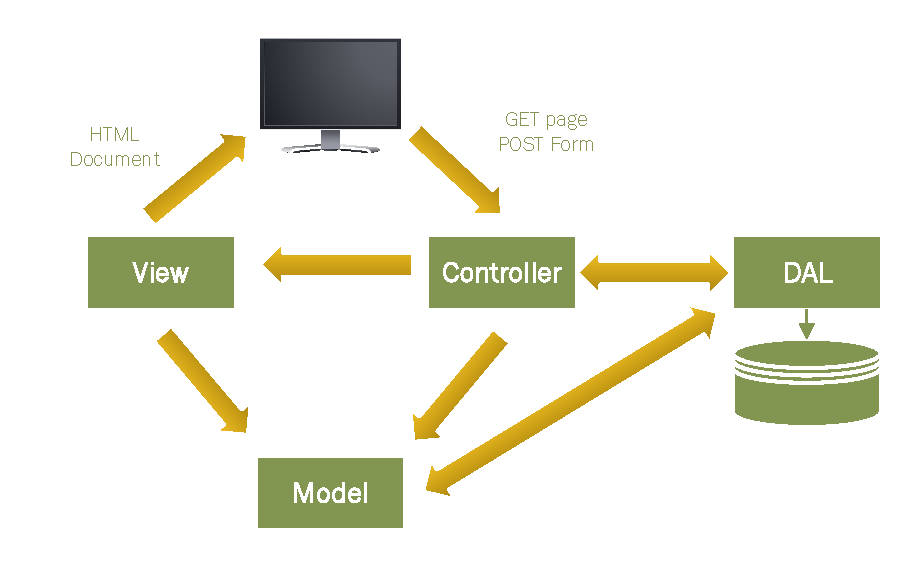
\includegraphics
	[width=140mm]{figures/MVC_drawing.pdf}
	\caption{MVC struktur}
	\label{fig:MVC}
\end{figure}

 \subsection{Data Access Layer}
 
 \subsubsection{Entity Framework}
 Entity framework (EF) var det oplagte valg når først ASP.NET MVC var valgt. EF kommer som standard når der oprettes et ASP.NET MVC projekt, og opretter selv en skabelon til at oprette database tabeller. EF er et object-relational mapping (ORM) framework til ADO.NET, der understøtter udviklingen af data orienterede applikationer. Hvilket vil sige at EF sørger for en nem adgang til den database man anvender til at gemme og hente data til viewet. \\
 \noindent Til selve databasen er der anvendt SQL Server 2016, som IHA har stillet til rådighed.
 
 \subsection{Presentation Layer}
 Til præsentations laget anvendes der HTML/CSS til at præsentere data for brugeren. For at gøre webapplikationen så skalerbart som muligt er der anvendt Bootstrap som framework. Dette framework gør det nemt at designe et View der kan skaleres til en hvilken som helst skærm - hvad end om det er mobil, tablet eller desktop. Desuden indeholder Bootstrap en række temaer, der gør det enkelt at designe et View der er pænt, hvilket ikke gruppens stærke side. \\
 For at gøre View'et mere dynamisk er der anvendt Javascript - mere specifikt JQuery. Dette bibliotek gør det muligt fx at vise popup vinduer, hvis der er brug for det eller i gruppens tilfælde at kunne bedømme en anden bruger.